\documentclass{article}

% content/resources/templates/preamble.tex
\usepackage[margin=0.6in]{geometry}
\author{Milav Dabgar}
\usepackage{amsmath,amssymb,amsthm}
\usepackage{booktabs}
\usepackage{multirow}
\usepackage{xcolor}
\usepackage{tcolorbox}
\tcbuselibrary{breakable,skins}
\usepackage[colorlinks=true,linkcolor=blue]{hyperref}
\usepackage{titlesec}
\usepackage{enumitem}
\usepackage{tikz}
\usepackage{pgfplots}
\usepackage{circuitikz}
\usepackage[version=4]{mhchem}
\usepackage{longtable}
\usepackage{array}
\usepackage{float}
\usepackage{caption}
\usepackage{listings}

\lstset{
  basicstyle=\small\ttfamily,
  breaklines=true,
  breakatwhitespace=false,
  postbreak=\mbox{\textcolor{red}{$\hookrightarrow$}\space},
  float=false,
  numbers=left,
  numberstyle=\tiny\color{gray},
  numbersep=10pt,
  xleftmargin=2em,
  keywordstyle=\color{blue},
  commentstyle=\color{green!60!black},
  stringstyle=\color{purple},
  backgroundcolor=\color{gray!5},
  showstringspaces=false,
  tabsize=2,
  captionpos=b,
  keepspaces=true,
  columns=flexible
}

\pgfplotsset{compat=1.18}
\usetikzlibrary{shapes,arrows,positioning,calc,patterns,decorations.pathmorphing,decorations.markings,arrows.meta}

% Color scheme
\definecolor{headcolor}{RGB}{0,102,204}
\definecolor{keycolor}{RGB}{220,20,60}
\definecolor{solutioncolor}{RGB}{34,139,34}
\definecolor{mnemoniccolor}{RGB}{148,0,211}
\definecolor{codecolor}{RGB}{0,0,100}

% Spacing
\setlength{\parskip}{3pt}
\setlist[itemize]{nosep}
\setlist[enumerate]{nosep}

% Title formatting
\titleformat{\section}{\Large\bfseries\color{headcolor}}{\thesection}{1em}{}
\titleformat{\subsection}{\large\bfseries\color{headcolor}}{\thesubsection}{1em}{}

% Pandoc tightlist compatibility
\providecommand{\tightlist}{%
  \setlength{\itemsep}{0pt}\setlength{\parskip}{0pt}}

% Pandoc longtable compatibility
\newcounter{none}
\def\thenone{}


% content/resources/templates/english-boxes.tex

% Custom environments
\newtcolorbox{solutionbox}{
 breakable,
 enhanced,
 colback=solutioncolor!5!white,
 colframe=solutioncolor!75!black,
 fonttitle=\bfseries,
 title=Solution
}

\newtcolorbox{solutionboxnobreak}{
 colback=solutioncolor!5!white,
 colframe=solutioncolor!75!black,
 fonttitle=\bfseries,
 title=Solution
}

\newtcolorbox{keyformula}{
 breakable,
 enhanced,
 colback=keycolor!5!white,
 colframe=keycolor!75!black,
 fonttitle=\bfseries,
 title=Key Formula
}

\newtcolorbox{mnemonicboxenv}{
 breakable,
 enhanced,
 colback=mnemoniccolor!5!white,
 colframe=mnemoniccolor!75!black,
 fonttitle=\bfseries,
 title=Mnemonic
}

\newcommand{\mnemonicbox}[1]{%
  \begin{mnemonicboxenv}
    #1
  \end{mnemonicboxenv}
}


% Custom commands for GTU solutions
% This file defines semantic commands for consistent formatting

% Question command with automatic formatting
\newcommand{\question}[2]{%
  \section*{Question #1}%
  \textbf{#2}%
}

% OR question variant
\newcommand{\questionor}[2]{%
  \section*{Question #1 OR}%
  \textbf{#2}%
}

% Proper table environment with caption
\newenvironment{answertable}[1]{%
  \begin{table}[htbp]
  \centering
  \caption{#1}
}{%
  \end{table}
}

% Proper figure environment for diagrams
\newenvironment{answerdiagram}[1]{%
  \begin{figure}[htbp]
  \centering
  \caption{#1}
}{%
  \end{figure}
}

% Semantic markup for key terms
\newcommand{\keyword}[1]{\textbf{#1}}
\newcommand{\code}[1]{\texttt{#1}}
\newcommand{\classname}[1]{\texttt{#1}}
\newcommand{\methodname}[1]{\texttt{#1}}

% Proper quotation marks
\newcommand{\mnemonic}[1]{``#1''}


\title{Fundamentals of Software Development (4331604) - Summer 2024 Solution}
\date{June 14, 2024}

\begin{document}
\maketitle

\questionmarks{1(a)}{3}{Explain software engineering layered approach.}

\begin{solutionbox}
Software engineering follows a layered approach with four fundamental layers working together to create quality software products.

\begin{center}
\captionof{table}{Software Engineering Layered Approach}
\begin{tabulary}{\linewidth}{|L|L|L|}
\hline
\textbf{Layer} & \textbf{Description} & \textbf{Purpose} \\ \hline
\textbf{Quality Focus} & Foundation layer emphasizing continuous improvement & Ensures defect-free products \\ \hline
\textbf{Process} & Defines framework of activities and tasks & Provides systematic development approach \\ \hline
\textbf{Methods} & Technical procedures for analysis, design, coding, testing & Offers ``how-to'' guidance \\ \hline
\textbf{Tools} & Automated support for process and methods & Provides efficiency and consistency \\ \hline
\end{tabulary}
\end{center}

\begin{itemize}
    \item \keyword{Quality Focus}: Forms the foundation ensuring customer satisfaction
    \item \keyword{Process Layer}: Defines workflow and project management activities
    \item \keyword{Methods Layer}: Provides technical approach for each development phase
    \item \keyword{Tools Layer}: Supports automation and integration
\end{itemize}
\end{solutionbox}

\begin{mnemonicbox}
\mnemonic{Quality Processes Make Tools: Remember the four layers from bottom to top.}
\end{mnemonicbox}

\questionmarks{1(b)}{4}{Explain Iterative waterfall model.}

\begin{solutionbox}
The Iterative Waterfall Model combines the structured approach of waterfall with feedback loops for improvement and error correction.

\begin{center}
\begin{tikzpicture}[node distance=1.5cm, auto, every node/.style={gtu state, align=center}]
    \node (Req) {Requirements\\Analysis};
    \node [right=of Req] (Sys) {System\\Design};
    \node [right=of Sys] (Imp) {Implementation};
    \node [below=of Imp] (Int) {Integration \&\\Testing};
    \node [left=of Int] (Dep) {Deployment};
    \node [left=of Dep] (Mai) {Maintenance};

    \path [gtu arrow] (Req) -- (Sys);
    \path [gtu arrow] (Sys) -- (Imp);
    \path [gtu arrow] (Imp) -- (Int);
    \path [gtu arrow] (Int) -- (Dep);
    \path [gtu arrow] (Dep) -- (Mai);

    % Feedback loops
    \path [gtu arrow, dashed, bend left] (Sys) to node [above, font=\footnotesize] {Feedback} (Req);
    \path [gtu arrow, dashed, bend left] (Imp) to node [above, font=\footnotesize] {Feedback} (Sys);
    \path [gtu arrow, dashed, bend left] (Int) to node [right, font=\footnotesize] {Feedback} (Imp);
    \path [gtu arrow, dashed, bend left] (Dep) to node [below, font=\footnotesize] {Feedback} (Int);
    \path [gtu arrow, dashed, bend left] (Mai) to node [below, font=\footnotesize] {Feedback} (Dep);
\end{tikzpicture}
\captionof{figure}{Iterative Waterfall Model}
\end{center}

\textbf{Key Features:}
\begin{itemize}
    \item \keyword{Sequential phases}: Each phase completed before next begins
    \item \keyword{Feedback loops}: Allow return to previous phases for corrections
    \item \keyword{Documentation driven}: Heavy emphasis on documentation at each phase
    \item \keyword{Error correction}: Issues identified in later phases can be fixed
\end{itemize}
\end{solutionbox}

\begin{mnemonicbox}
\mnemonic{Water Falls Back Up: Sequential flow with upward feedback capability.}
\end{mnemonicbox}

\questionmarks{1(c)}{7}{Explain Agile Model and Agile Principles.}

\begin{solutionbox}
Agile is an iterative software development methodology emphasizing collaboration, customer feedback, and rapid delivery of working software.

\begin{center}
\captionof{table}{Agile Values vs Traditional Approach}
\begin{tabulary}{\linewidth}{|L|L|}
\hline
\textbf{Agile Values} & \textbf{Traditional Approach} \\ \hline
Individuals and interactions & Processes and tools \\ \hline
Working software & Comprehensive documentation \\ \hline
Customer collaboration & Contract negotiation \\ \hline
Responding to change & Following a plan \\ \hline
\end{tabulary}
\end{center}

\textbf{Core Agile Principles:}
\begin{itemize}
    \item \keyword{Customer satisfaction}: Deliver valuable software early and continuously
    \item \keyword{Welcome change}: Embrace changing requirements even late in development
    \item \keyword{Frequent delivery}: Deliver working software frequently (weeks rather than months)
    \item \keyword{Collaboration}: Business people and developers work together daily
    \item \keyword{Motivated individuals}: Build projects around motivated people
    \item \keyword{Face-to-face conversation}: Most efficient method of communication
    \item \keyword{Working software}: Primary measure of progress
    \item \keyword{Sustainable development}: Maintain constant pace indefinitely
    \item \keyword{Technical excellence}: Continuous attention to good design
    \item \keyword{Simplicity}: Art of maximizing work not done
    \item \keyword{Self-organizing teams}: Best requirements emerge from self-organizing teams
    \item \keyword{Regular reflection}: Team reflects and adjusts behavior regularly
\end{itemize}

\begin{center}
\begin{tikzpicture}[node distance=2cm, auto, every node/.style={gtu state, align=center, font=\small}]
    \node (Plan) {Planning};
    \node [right=of Plan] (Des) {Design};
    \node [right=of Des] (Code) {Coding};
    \node [below=of Code] (Test) {Testing};
    \node [left=of Test] (Rev) {Review};
    \node [left=of Rev] (Rel) {Release};

    \path [gtu arrow] (Plan) -- (Des);
    \path [gtu arrow] (Des) -- (Code);
    \path [gtu arrow] (Code) -- (Test);
    \path [gtu arrow] (Test) -- (Rev);
    \path [gtu arrow] (Rev) -- (Plan);
    \path [gtu arrow] (Rev) -- (Rel);
\end{tikzpicture}
\captionof{figure}{Agile Development Cycle}
\end{center}
\end{solutionbox}

\begin{mnemonicbox}
\mnemonic{Customer Change Frequently Collaborates: Core agile principles focus.}
\end{mnemonicbox}

\questionmarks{1(c OR)}{7}{Write a short note on Scrum.}

\begin{solutionbox}
Scrum is an agile framework for managing software development with emphasis on team collaboration and iterative progress.

\begin{center}
\captionof{table}{Scrum Roles and Responsibilities}
\begin{tabulary}{\linewidth}{|L|L|L|}
\hline
\textbf{Role} & \textbf{Responsibilities} & \textbf{Key Activities} \\ \hline
\textbf{Product Owner} & Defines product features and priorities & Manages product backlog \\ \hline
\textbf{Scrum Master} & Facilitates process and removes obstacles & Conducts ceremonies \\ \hline
\textbf{Development Team} & Creates working software & Self-organizing and cross-functional \\ \hline
\end{tabulary}
\end{center}

\textbf{Scrum Events:}
\begin{itemize}
    \item \keyword{Sprint}: 1-4 week iteration producing potentially shippable product
    \item \keyword{Sprint Planning}: Team plans work for upcoming sprint
    \item \keyword{Daily Scrum}: 15-minute daily synchronization meeting
    \item \keyword{Sprint Review}: Demonstrate completed work to stakeholders
    \item \keyword{Sprint Retrospective}: Team reflects on process improvements
\end{itemize}

\textbf{Scrum Artifacts:}
\begin{itemize}
    \item \keyword{Product Backlog}: Prioritized list of features
    \item \keyword{Sprint Backlog}: Items selected for current sprint
    \item \keyword{Increment}: Working product at sprint end
\end{itemize}

\begin{center}
\begin{tikzpicture}[node distance=1.5cm, auto, every node/.style={gtu block, align=center, font=\small}]
    \node (Backlogs) {Product\\Backlog};
    \node [right=of Backlogs] (Plan) {Sprint\\Planning};
    \node [right=of Plan] (SprintBack) {Sprint\\Backlog};
    \node [below=of SprintBack] (Daily) {Daily\\Scrum};
    \node [left=of Daily] (Review) {Sprint\\Review};
    \node [left=of Review] (Retro) {Sprint\\Retrospective};
    \node [below=of Review] (Inc) {Product\\Increment};

    \path [gtu arrow] (Backlogs) -- (Plan);
    \path [gtu arrow] (Plan) -- (SprintBack);
    \path [gtu arrow] (SprintBack) -- (Daily);
    \path [gtu arrow] (Daily) -- (Review);
    \path [gtu arrow] (Review) -- (Retro);
    \path [gtu arrow] (Retro) |- (Plan);
    \path [gtu arrow] (Review) -- (Inc);
\end{tikzpicture}
\captionof{figure}{Scrum Process Flow}
\end{center}
\end{solutionbox}

\begin{mnemonicbox}
\mnemonic{Product Sprints Daily Reviews: Key scrum elements sequence.}
\end{mnemonicbox}

\questionmarks{2(a)}{3}{If you have to develop a word processing software product, what process models will you choose? Justify your answer.}

\begin{solutionbox}
For word processing software development, I would choose the \keyword{Incremental Model} as the most suitable process model.

\textbf{Justification:}
\begin{itemize}
    \item \keyword{Complex functionality}: Word processors have numerous features (editing, formatting, spell-check) that can be developed incrementally
    \item \keyword{User feedback}: Early increments allow user testing and feedback incorporation
    \item \keyword{Risk management}: Core features delivered first, advanced features added later
    \item \keyword{Market advantage}: Basic version can be released early to gain market presence
\end{itemize}

\textbf{Development Increments:}
\begin{enumerate}
    \item \textbf{Increment 1}: Basic text editing and file operations
    \item \textbf{Increment 2}: Formatting and font management
    \item \textbf{Increment 3}: Advanced features (spell-check, templates)
\end{enumerate}
\end{solutionbox}

\begin{mnemonicbox}
\mnemonic{Word Processing Increments User Feedback: Incremental approach suits complex software.}
\end{mnemonicbox}

\questionmarks{2(b)}{4}{Explain characteristics of good SRS.}

\begin{solutionbox}
A good Software Requirements Specification (SRS) document must possess specific characteristics to ensure successful software development.

\begin{center}
\captionof{table}{Characteristics of Good SRS}
\begin{tabulary}{\linewidth}{|L|L|L|}
\hline
\textbf{Characteristic} & \textbf{Description} & \textbf{Importance} \\ \hline
\textbf{Complete} & Contains all necessary requirements & Prevents scope creep \\ \hline
\textbf{Consistent} & No conflicting requirements & Avoids implementation confusion \\ \hline
\textbf{Unambiguous} & Clear and precise language & Single interpretation possible \\ \hline
\textbf{Verifiable} & Requirements can be tested & Enables validation \\ \hline
\textbf{Modifiable} & Easy to change and maintain & Supports requirement evolution \\ \hline
\textbf{Traceable} & Requirements linked to sources & Impact analysis possible \\ \hline
\end{tabulary}
\end{center}

\textbf{Additional Characteristics:}
\begin{itemize}
    \item \keyword{Feasible}: Technically and economically achievable
    \item \keyword{Necessary}: Each requirement serves a purpose
    \item \keyword{Prioritized}: Requirements ranked by importance
    \item \keyword{Testable}: Specific criteria for verification
\end{itemize}
\end{solutionbox}

\begin{mnemonicbox}
\mnemonic{Complete Consistent Unambiguous Verifiable: Core SRS quality attributes.}
\end{mnemonicbox}

\questionmarks{2(c)}{7}{Explain functional and non-functional requirements for an ATM software.}

\begin{solutionbox}
ATM software requirements are categorized into functional (what system does) and non-functional (how system performs) requirements.

\begin{center}
\captionof{table}{ATM Functional Requirements}
\begin{tabulary}{\linewidth}{|L|L|L|}
\hline
\textbf{Function} & \textbf{Description} & \textbf{Example} \\ \hline
\textbf{Authentication} & User login and verification & PIN validation, card reading \\ \hline
\textbf{Account Operations} & Basic banking transactions & Balance inquiry, cash withdrawal \\ \hline
\textbf{Transaction Processing} & Money transfer and deposits & Account-to-account transfer \\ \hline
\textbf{Receipt Generation} & Transaction documentation & Print transaction receipts \\ \hline
\textbf{Session Management} & User session control & Timeout, logout functionality \\ \hline
\end{tabulary}
\end{center}

\begin{center}
\captionof{table}{ATM Non-Functional Requirements}
\begin{tabulary}{\linewidth}{|L|L|L|}
\hline
\textbf{Category} & \textbf{Requirement} & \textbf{Specification} \\ \hline
\textbf{Performance} & Response time & Maximum 3 seconds per transaction \\ \hline
\textbf{Security} & Data protection & 256-bit encryption for all data \\ \hline
\textbf{Reliability} & System availability & 99.9\% uptime requirement \\ \hline
\textbf{Usability} & User interface & Simple interface for all age groups \\ \hline
\textbf{Scalability} & Load handling & Support 1000 concurrent users \\ \hline
\end{tabulary}
\end{center}

\textbf{Functional Requirements Details:}
\begin{itemize}
    \item \keyword{Cash Withdrawal}: Dispense cash after successful authentication
    \item \keyword{Balance Inquiry}: Display current account balance
    \item \keyword{PIN Change}: Allow users to update their PIN
    \item \keyword{Mini Statement}: Provide last 10 transactions
\end{itemize}

\textbf{Non-Functional Requirements Details:}
\begin{itemize}
    \item \keyword{Security}: Multi-factor authentication, transaction logging
    \item \keyword{Performance}: Fast transaction processing, minimal wait time
    \item \keyword{Availability}: 24/7 operation with minimal downtime
    \item \keyword{Maintainability}: Easy software updates and hardware maintenance
\end{itemize}
\end{solutionbox}

\begin{mnemonicbox}
\mnemonic{Functions Work, Quality Matters: Functional vs non-functional distinction.}
\end{mnemonicbox}

\questionmarks{2(a OR)}{3}{Explain Incremental Model with diagram.}

\begin{solutionbox}
The Incremental Model develops software in small, manageable portions called increments, with each increment adding new functionality to the existing system.

\begin{center}
\begin{tikzpicture}[node distance=1.5cm, auto, every node/.style={gtu block, font=\small}]
    \node (Req) {Requirements};
    
    \node [right=2cm of Req] (Inc1) {Increment 1};
    \node [below=of Inc1] (Inc2) {Increment 2};
    \node [below=of Inc2] (Inc3) {Increment 3};

    \path [gtu arrow] (Req) -- (Inc1);
    \path [gtu arrow] (Req) |- (Inc2);
    \path [gtu arrow] (Req) |- (Inc3);

    % Details for Inc 1
    \node [right=1cm of Inc1, gtu state] (Rel1) {Release 1};
    \path [gtu arrow] (Inc1) -- node[above, font=\tiny]{Design, Code, Test} (Rel1);
    
    % Details for Inc 2
    \node [right=1cm of Inc2, gtu state] (Rel2) {Release 2};
    \path [gtu arrow] (Inc2) -- node[above, font=\tiny]{Design, Code, Test} (Rel2);
    
    % Details for Inc 3
    \node [right=1cm of Inc3, gtu state] (Rel3) {Final Release};
    \path [gtu arrow] (Inc3) -- node[above, font=\tiny]{Design, Code, Test} (Rel3);

\end{tikzpicture}
\captionof{figure}{Incremental Model}
\end{center}

\textbf{Key Features:}
\begin{itemize}
    \item \keyword{Parallel development}: Multiple increments developed simultaneously
    \item \keyword{Early delivery}: Working software available after first increment
    \item \keyword{Risk reduction}: Core functionality delivered first
\end{itemize}
\end{solutionbox}

\begin{mnemonicbox}
\mnemonic{Increments Build Upon Previous: Each increment adds to existing functionality.}
\end{mnemonicbox}

\questionmarks{2(b OR)}{4}{Differentiate between functional and non-functional requirements.}

\begin{solutionbox}
\begin{center}
\captionof{table}{Functional vs Non-Functional Requirements}
\begin{tabulary}{\linewidth}{|L|L|L|}
\hline
\textbf{Aspect} & \textbf{Functional Requirements} & \textbf{Non-Functional Requirements} \\ \hline
\textbf{Definition} & What the system does & How the system performs \\ \hline
\textbf{Focus} & System behavior and features & System quality attributes \\ \hline
\textbf{Testing} & Black-box testing & Performance and stress testing \\ \hline
\textbf{Documentation} & Use cases, user stories & Quality metrics, constraints \\ \hline
\textbf{Examples} & Login, search, calculate & Speed, security, usability \\ \hline
\textbf{Verification} & Functional testing & Non-functional testing \\ \hline
\textbf{Change Impact} & Feature modification & Performance tuning \\ \hline
\textbf{User Visibility} & Directly visible to users & Indirectly experienced \\ \hline
\end{tabulary}
\end{center}

\textbf{Functional Requirements Characteristics:}
\begin{itemize}
    \item \keyword{Behavior-focused}: Define system actions and responses
    \item \keyword{Feature-specific}: Each requirement describes a specific capability
    \item \keyword{User-driven}: Based on user needs and business processes
\end{itemize}

\textbf{Non-Functional Requirements Characteristics:}
\begin{itemize}
    \item \keyword{Quality-focused}: Define performance and quality standards
    \item \keyword{System-wide}: Apply to entire system rather than specific features
    \item \keyword{Constraint-driven}: Set limits and boundaries for system operation
\end{itemize}
\end{solutionbox}

\begin{mnemonicbox}
\mnemonic{Functions Do, Quality Shows: Functional requirements define actions, non-functional define quality.}
\end{mnemonicbox}

\questionmarks{2(c OR)}{7}{Write a short note on Requirements Analysis.}

\begin{solutionbox}
Requirements Analysis is the process of studying user needs and defining system requirements to understand what the software system should accomplish.

\begin{center}
\captionof{table}{Requirements Analysis Process}
\begin{tabulary}{\linewidth}{|L|L|L|}
\hline
\textbf{Phase} & \textbf{Activities} & \textbf{Deliverables} \\ \hline
\textbf{Elicitation} & Gather requirements from stakeholders & Requirement lists, interviews \\ \hline
\textbf{Analysis} & Study and understand requirements & Requirement models, prototypes \\ \hline
\textbf{Specification} & Document requirements formally & SRS document, use cases \\ \hline
\textbf{Validation} & Verify requirements correctness & Validated requirements \\ \hline
\end{tabulary}
\end{center}

\textbf{Requirements Elicitation Techniques:}
\begin{itemize}
    \item \keyword{Interviews}: One-on-one discussions with stakeholders
    \item \keyword{Questionnaires}: Structured surveys for large user groups
    \item \keyword{Observation}: Studying current work processes
    \item \keyword{Workshops}: Group sessions for requirement gathering
    \item \keyword{Prototyping}: Building preliminary versions for feedback
\end{itemize}

\textbf{Analysis Activities:}
\begin{itemize}
    \item \keyword{Requirement prioritization}: Ranking requirements by importance
    \item \keyword{Feasibility study}: Assessing technical and economic viability
    \item \keyword{Conflict resolution}: Resolving contradictory requirements
    \item \keyword{Requirement modeling}: Creating visual representations
\end{itemize}

\textbf{Validation Techniques:}
\begin{itemize}
    \item \keyword{Requirement reviews}: Formal examination of documented requirements
    \item \keyword{Prototyping}: Building models to validate understanding
    \item \keyword{Test case generation}: Creating tests from requirements
\end{itemize}

\textbf{Challenges in Requirements Analysis:}
\begin{itemize}
    \item \keyword{Changing requirements}: Stakeholder needs evolve over time
    \item \keyword{Communication gaps}: Misunderstanding between users and developers
    \item \keyword{Incomplete requirements}: Missing or vague specifications
    \item \keyword{Conflicting stakeholder needs}: Different user groups have different priorities
\end{itemize}
\end{solutionbox}

\begin{mnemonicbox}
\mnemonic{Every Analysis Specification Validates: Key phases of requirements analysis.}
\end{mnemonicbox}

\questionmarks{3(a)}{3}{Explain Gantt Chart.}

\begin{solutionbox}
A Gantt Chart is a visual project management tool that displays project tasks against a timeline, showing task duration, dependencies, and progress.

\begin{center}
\captionof{table}{Gantt Chart Components}
\begin{tabulary}{\linewidth}{|L|L|L|}
\hline
\textbf{Component} & \textbf{Description} & \textbf{Purpose} \\ \hline
\textbf{Tasks} & Project activities listed vertically & Shows work breakdown \\ \hline
\textbf{Timeline} & Horizontal time scale & Displays project duration \\ \hline
\textbf{Bars} & Horizontal bars showing task duration & Visual task representation \\ \hline
\textbf{Dependencies} & Lines connecting related tasks & Shows task relationships \\ \hline
\textbf{Milestones} & Key project checkpoints & Marks important events \\ \hline
\end{tabulary}
\end{center}

\begin{center}
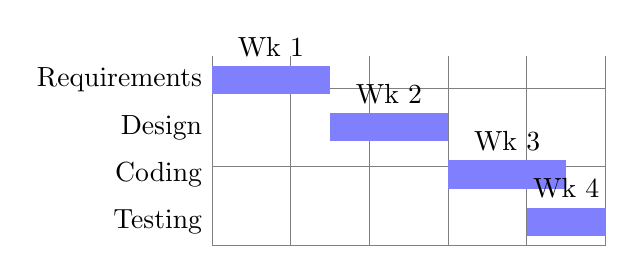
\begin{tikzpicture}[x=1cm, y=0.6cm]
    \draw[help lines] (0,0) grid (5,4);
    
    \node[anchor=east] at (0,3.5) {Requirements};
    \node[anchor=east] at (0,2.5) {Design};
    \node[anchor=east] at (0,1.5) {Coding};
    \node[anchor=east] at (0,0.5) {Testing};

    \fill[blue!50] (0,3.2) rectangle (1.5,3.8);
    \fill[blue!50] (1.5,2.2) rectangle (3,2.8);
    \fill[blue!50] (3,1.2) rectangle (4.5,1.8);
    \fill[blue!50] (4,0.2) rectangle (5,0.8);
    
    \node[anchor=south] at (0.75,3.8) {Wk 1};
    \node[anchor=south] at (2.25,2.8) {Wk 2};
    \node[anchor=south] at (3.75,1.8) {Wk 3};
    \node[anchor=south] at (4.5,0.8) {Wk 4};

\end{tikzpicture}
\captionof{figure}{Sample Gantt Chart}
\end{center}

\textbf{Benefits:}
\begin{itemize}
    \item \keyword{Visual clarity}: Easy to understand project timeline
    \item \keyword{Progress tracking}: Shows completed vs remaining work
    \item \keyword{Resource planning}: Helps allocate resources effectively
\end{itemize}
\end{solutionbox}

\begin{mnemonicbox}
\mnemonic{Gantt Graphs Timeline Tasks: Visual timeline representation of project tasks.}
\end{mnemonicbox}

\questionmarks{3(b)}{4}{Write in brief: Responsibilities and skills of software project manager.}

\begin{solutionbox}
A software project manager oversees the entire software development lifecycle, ensuring projects are completed on time, within budget, and meet quality standards.

\begin{center}
\captionof{table}{Project Manager Responsibilities}
\begin{tabulary}{\linewidth}{|L|L|L|}
\hline
\textbf{Category} & \textbf{Responsibilities} & \textbf{Key Activities} \\ \hline
\textbf{Planning} & Project scope and timeline definition & WBS creation, scheduling \\ \hline
\textbf{Resource Management} & Team allocation and coordination & Staff assignment, skill matching \\ \hline
\textbf{Risk Management} & Identify and mitigate project risks & Risk assessment, contingency planning \\ \hline
\textbf{Communication} & Stakeholder coordination & Status reporting, meetings \\ \hline
\textbf{Quality Assurance} & Ensure deliverable quality & Review processes, standards \\ \hline
\end{tabulary}
\end{center}

\textbf{Essential Skills:}
\begin{itemize}
    \item \keyword{Technical skills}: Understanding of software development processes
    \item \keyword{Leadership skills}: Team motivation and guidance
    \item \keyword{Communication skills}: Effective stakeholder interaction
    \item \keyword{Problem-solving skills}: Quick issue resolution
    \item \keyword{Time management}: Efficient task prioritization
\end{itemize}

\textbf{Key Responsibilities:}
\begin{itemize}
    \item \keyword{Project planning}: Define scope, timeline, and resources
    \item \keyword{Team coordination}: Manage development team activities
    \item \keyword{Stakeholder management}: Maintain client and sponsor relationships
    \item \keyword{Risk mitigation}: Identify and address potential problems
\end{itemize}
\end{solutionbox}

\begin{mnemonicbox}
\mnemonic{Managers Plan Resources Risks Communication: Core responsibilities of project managers.}
\end{mnemonicbox}

\questionmarks{3(c)}{7}{Write a short note on Risk Management.}

\begin{solutionbox}
Risk Management is the systematic process of identifying, analyzing, and responding to project risks that could impact software development success.

\begin{center}
\captionof{table}{Risk Management Process}
\begin{tabulary}{\linewidth}{|L|L|L|L|}
\hline
\textbf{Phase} & \textbf{Activities} & \textbf{Techniques} & \textbf{Outcomes} \\ \hline
\textbf{Risk Identification} & Find potential risks & Brainstorming, checklists & Risk register \\ \hline
\textbf{Risk Analysis} & Assess probability and impact & Risk matrices, scoring & Prioritized risks \\ \hline
\textbf{Risk Planning} & Develop response strategies & Mitigation, avoidance & Risk response plans \\ \hline
\textbf{Risk Monitoring} & Track and control risks & Regular reviews & Updated risk status \\ \hline
\end{tabulary}
\end{center}

\textbf{Types of Software Project Risks:}

\textbf{Technical Risks:}
\begin{itemize}
    \item \keyword{Technology uncertainty}: New or unproven technologies
    \item \keyword{Performance issues}: System not meeting performance requirements
    \item \keyword{Integration problems}: Difficulty combining system components
\end{itemize}

\textbf{Project Risks:}
\begin{itemize}
    \item \keyword{Schedule delays}: Tasks taking longer than estimated
    \item \keyword{Resource constraints}: Insufficient staff or budget
    \item \keyword{Scope creep}: Uncontrolled requirement changes
\end{itemize}

\textbf{Business Risks:}
\begin{itemize}
    \item \keyword{Market changes}: Shifting business requirements
    \item \keyword{Competition}: Competitive products affecting project value
    \item \keyword{Regulatory changes}: New compliance requirements
\end{itemize}

\textbf{Risk Response Strategies:}
\begin{itemize}
    \item \keyword{Risk Avoidance}: Eliminate risk by changing project approach
    \item \keyword{Risk Mitigation}: Reduce probability or impact of risk
    \item \keyword{Risk Transfer}: Shift risk to third party (insurance, outsourcing)
    \item \keyword{Risk Acceptance}: Accept risk and develop contingency plans
\end{itemize}
\end{solutionbox}

\begin{mnemonicbox}
\mnemonic{Identify Analyze Plan Monitor: Four phases of risk management process.}
\end{mnemonicbox}

\questionmarks{3(a OR)}{3}{Explain WBS with example.}

\begin{solutionbox}
Work Breakdown Structure (WBS) is a hierarchical decomposition of project work into smaller, manageable components that can be easily estimated, assigned, and tracked.

\begin{center}
\begin{tikzpicture}[level 1/.style={sibling distance=3cm}, level 2/.style={sibling distance=1.5cm}, nodes={gtu block, draw, minimum height=0.6cm, align=center, font=\scriptsize}]
    \node {E-commerce\\Website}
        child { node {Frontend\\Development}
            child { node {UI} }
            child { node {Cart} }
            child { node {Payment} }
        }
        child { node {Backend\\Development}
            child { node {DB} }
            child { node {User} }
            child { node {Orders} }
        }
        child { node {Testing}
            child { node {Unit} }
            child { node {Integration} }
        }
        child { node {Deployment} };
\end{tikzpicture}
\captionof{figure}{WBS Example for E-commerce Website}
\end{center}

\textbf{WBS Characteristics:}
\begin{itemize}
    \item \keyword{Hierarchical structure}: Top-down breakdown of project scope
    \item \keyword{100\% rule}: WBS includes 100\% of work defined by project scope
    \item \keyword{Mutually exclusive}: No overlap between WBS elements
\end{itemize}
\end{solutionbox}

\begin{mnemonicbox}
\mnemonic{Work Breaks Small: Breaking work into smaller manageable pieces.}
\end{mnemonicbox}

\questionmarks{3(b OR)}{4}{Explain Project monitoring and control.}

\begin{solutionbox}
Project monitoring and control involves tracking project progress, comparing actual performance against planned performance, and taking corrective actions when necessary.

\begin{center}
\captionof{table}{Monitoring and Control Activities}
\begin{tabulary}{\linewidth}{|L|L|L|}
\hline
\textbf{Activity} & \textbf{Description} & \textbf{Tools/Techniques} \\ \hline
\textbf{Progress Tracking} & Monitor task completion & Gantt charts, dashboards \\ \hline
\textbf{Performance Measurement} & Compare actual vs planned & Earned value analysis \\ \hline
\textbf{Quality Control} & Ensure deliverable quality & Reviews, testing \\ \hline
\textbf{Risk Monitoring} & Track identified risks & Risk registers, reports \\ \hline
\textbf{Change Control} & Manage scope changes & Change request process \\ \hline
\end{tabulary}
\end{center}

\textbf{Key Monitoring Metrics:}
\begin{itemize}
    \item \keyword{Schedule performance}: Tasks completed on time
    \item \keyword{Cost performance}: Budget utilization and variance
    \item \keyword{Quality metrics}: Defect rates, customer satisfaction
    \item \keyword{Resource utilization}: Team productivity and efficiency
\end{itemize}

\textbf{Control Actions:}
\begin{itemize}
    \item \keyword{Corrective actions}: Address performance deviations
    \item \keyword{Preventive actions}: Avoid potential problems
    \item \keyword{Change management}: Handle scope modifications
\end{itemize}
\end{solutionbox}

\begin{mnemonicbox}
\mnemonic{Monitor Progress Performance Quality: Key areas of project monitoring.}
\end{mnemonicbox}

\questionmarks{3(c OR)}{7}{Explain Critical Path Method (CPM) with a suitable example.}

\begin{solutionbox}
Critical Path Method (CPM) is a project management technique that identifies the longest sequence of dependent tasks and determines the minimum project completion time.

\begin{center}
\captionof{table}{Sample Project Tasks}
\begin{tabulary}{\linewidth}{|L|L|L|}
\hline
\textbf{Task} & \textbf{Duration (Days)} & \textbf{Predecessors} \\ \hline
A - Requirements & 5 & - \\ \hline
B - Design & 8 & A \\ \hline
C - Database Setup & 6 & A \\ \hline
D - Frontend Coding & 10 & B \\ \hline
E - Backend Coding & 12 & B, C \\ \hline
F - Integration & 4 & D, E \\ \hline
G - Testing & 6 & F \\ \hline
\end{tabulary}
\end{center}

\begin{center}
\begin{tikzpicture}[node distance=1.5cm, auto, every node/.style={circle, draw, font=\small}]
    \node (A) {A:5};
    \node [above right=1cm and 1cm of A] (B) {B:8};
    \node [below right=1cm and 1cm of A] (C) {C:6};
    
    \node [right=1cm of B] (D) {D:10};
    \node [below right=1cm and 1cm of B] (E) {E:12};
    
    \node [right=1cm of E] (F) {F:4};
    \node [right=1cm of F] (G) {G:6};

    \path [gtu arrow] (A) -- (B);
    \path [gtu arrow] (A) -- (C);
    \path [gtu arrow] (B) -- (D);
    \path [gtu arrow] (B) -- (E);
    \path [gtu arrow] (C) -- (E);
    \path [gtu arrow] (D) -- (F);
    \path [gtu arrow] (E) -- (F);
    \path [gtu arrow] (F) -- (G);
\end{tikzpicture}
\captionof{figure}{CPM Network}
\end{center}

\textbf{Critical Path Calculation:}
\begin{itemize}
    \item \textbf{Path 1}: A $\to$ B $\to$ D $\to$ F $\to$ G = 5 + 8 + 10 + 4 + 6 = 33 days
    \item \textbf{Path 2}: A $\to$ B $\to$ E $\to$ F $\to$ G = 5 + 8 + 12 + 4 + 6 = 35 days (Critical Path)
    \item \textbf{Path 3}: A $\to$ C $\to$ E $\to$ F $\to$ G = 5 + 6 + 12 + 4 + 6 = 33 days
\end{itemize}

\textbf{CPM Benefits:}
\begin{itemize}
    \item \keyword{Project duration}: Determines minimum completion time
    \item \keyword{Critical activities}: Identifies tasks that cannot be delayed
    \item \keyword{Float calculation}: Shows available slack time for non-critical tasks
    \item \keyword{Resource optimization}: Helps allocate resources efficiently
\end{itemize}
\end{solutionbox}

\begin{mnemonicbox}
\mnemonic{Critical Paths Minimize Project Duration: CPM finds longest path determining minimum time.}
\end{mnemonicbox}

\questionmarks{4(a)}{3}{Write a note on classification of design activities.}

\begin{solutionbox}
Software design activities are systematically classified to organize the design process and ensure comprehensive system development.

\begin{center}
\captionof{table}{Classification of Design Activities}
\begin{tabulary}{\linewidth}{|L|L|L|}
\hline
\textbf{Classification} & \textbf{Activities} & \textbf{Focus Area} \\ \hline
\textbf{Architectural Design} & System structure, components & High-level organization \\ \hline
\textbf{Interface Design} & User interface, system interfaces & Interaction design \\ \hline
\textbf{Component Design} & Module details, algorithms & Low-level implementation \\ \hline
\textbf{Data Design} & Database, data structures & Data organization \\ \hline
\end{tabulary}
\end{center}

\textbf{Design Activity Levels:}
\begin{itemize}
    \item \keyword{System Level}: Overall system architecture and major components
    \item \keyword{Subsystem Level}: Individual subsystem design and interfaces
    \item \keyword{Component Level}: Detailed module design and algorithms
\end{itemize}
\end{solutionbox}

\begin{mnemonicbox}
\mnemonic{Architects Interface Components Data: Four main design activity classifications.}
\end{mnemonicbox}

\questionmarks{4(b)}{4}{Define Coupling. Explain its classification.}

\begin{solutionbox}
Coupling refers to the degree of interdependence between software modules. Lower coupling indicates better software design with more maintainable and flexible code.

\begin{center}
\captionof{table}{Types of Coupling (Loosest to Tightest)}
\begin{tabulary}{\linewidth}{|L|L|L|}
\hline
\textbf{Coupling Type} & \textbf{Description} & \textbf{Example} \\ \hline
\textbf{Data Coupling} & Modules communicate through parameters & Function calls with simple parameters \\ \hline
\textbf{Stamp Coupling} & Modules share composite data structure & Passing record/structure as parameter \\ \hline
\textbf{Control Coupling} & One module controls another's execution & Passing control flags \\ \hline
\textbf{External Coupling} & Modules depend on external format & Shared file format or protocol \\ \hline
\textbf{Common Coupling} & Modules share global data & Global variables access \\ \hline
\textbf{Content Coupling} & One module modifies another's data & Direct access to another module's data \\ \hline
\end{tabulary}
\end{center}

\textbf{Benefits of Loose Coupling:}
\begin{itemize}
    \item \keyword{Maintainability}: Easier to modify individual modules
    \item \keyword{Reusability}: Modules can be used in different contexts
    \item \keyword{Testability}: Modules can be tested independently
\end{itemize}
\end{solutionbox}

\begin{mnemonicbox}
\mnemonic{Data Stamp Control External Common Content: Coupling types from loose to tight.}
\end{mnemonicbox}

\questionmarks{4(c)}{7}{Draw a use case diagram for online shopping web application.}

\begin{solutionbox}
A use case diagram shows the functional requirements of an online shopping system by illustrating actors and their interactions with the system.

\begin{center}
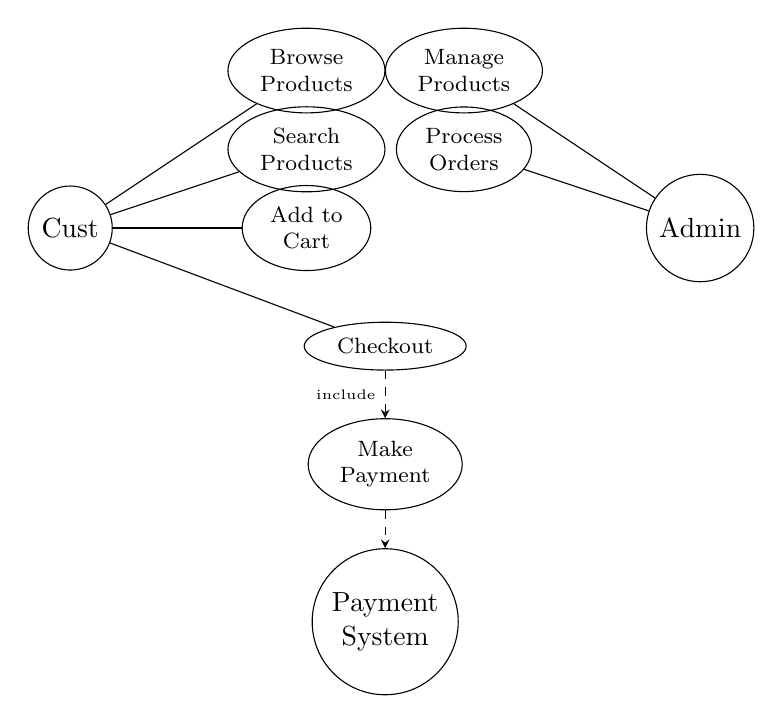
\begin{tikzpicture}[
    actor/.style={shape=circle, draw, align=center, minimum size=0.8cm},
    usecase/.style={shape=ellipse, draw, align=center, font=\footnotesize},
    edge/.style={->, >=stealth}
]
    % Actors
    \node[actor] (Cust) at (0, 0) {Cust};
    \node[actor] (Admin) at (8, 0) {Admin};
    \node[actor] (PaySys) at (4, -5) {Payment\\System};

    % Customer Use Cases
    \node[usecase] (Browse) at (3, 2) {Browse\\Products};
    \node[usecase] (Search) at (3, 1) {Search\\Products};
    \node[usecase] (Cart) at (3, 0) {Add to\\Cart};
    \node[usecase] (Checkout) at (4, -1.5) {Checkout};
    \node[usecase] (Payment) at (4, -3) {Make\\Payment};
    
    % Admin Use Cases
    \node[usecase] (ManageProd) at (5, 2) {Manage\\Products};
    \node[usecase] (ProcessOrder) at (5, 1) {Process\\Orders};

    % Connections
    \draw (Cust) -- (Browse);
    \draw (Cust) -- (Search);
    \draw (Cust) -- (Cart);
    \draw (Cust) -- (Checkout);
    
    \draw (Admin) -- (ManageProd);
    \draw (Admin) -- (ProcessOrder);
    
    \draw[edge, dashed] (Checkout) -- node[left, font=\tiny]{include} (Payment);
    \draw[edge, dashed] (Payment) -- (PaySys);

\end{tikzpicture}
\captionof{figure}{Online Shopping Use Case Diagram}
\end{center}

\textbf{Key Use Cases Explained:}

\textbf{Customer Use Cases:}
\begin{itemize}
    \item \keyword{Browse Products}: View available products by category
    \item \keyword{Search Products}: Find specific products using keywords
    \item \keyword{Shopping Cart}: Add, remove, and modify cart items
    \item \keyword{Checkout Process}: Complete purchase with shipping details
\end{itemize}

\textbf{Admin Use Cases:}
\begin{itemize}
    \item \keyword{Product Management}: Add, edit, delete products and categories
    \item \keyword{Order Processing}: Manage order fulfillment and shipping
\end{itemize}
\end{solutionbox}

\begin{mnemonicbox}
\mnemonic{Customers Browse Buy, Admins Manage Monitor: Core use case categories.}
\end{mnemonicbox}

\questionmarks{4(a OR)}{3}{Explain the characteristics of good UI.}

\begin{solutionbox}
Good User Interface (UI) design ensures effective user interaction with software systems through intuitive and user-friendly design principles.

\begin{center}
\captionof{table}{Characteristics of Good UI}
\begin{tabulary}{\linewidth}{|L|L|L|}
\hline
\textbf{Characteristic} & \textbf{Description} & \textbf{Example} \\ \hline
\textbf{Consistency} & Uniform design across application & Same button styles throughout \\ \hline
\textbf{Simplicity} & Easy to understand and use & Minimal, clean interface \\ \hline
\textbf{Visibility} & Important elements clearly visible & Key actions prominently displayed \\ \hline
\textbf{Feedback} & System responds to user actions & Progress bars, confirmations \\ \hline
\textbf{Error Prevention} & Prevents user mistakes & Input validation, confirmations \\ \hline
\textbf{Flexibility} & Accommodates different user needs & Customizable interfaces \\ \hline
\end{tabulary}
\end{center}

\textbf{UI Design Principles:}
\begin{itemize}
    \item \keyword{User-centered}: Design focused on user needs and goals
    \item \keyword{Accessibility}: Usable by people with different abilities
    \item \keyword{Efficiency}: Minimizes steps to complete tasks
\end{itemize}
\end{solutionbox}

\begin{mnemonicbox}
\mnemonic{Consistent Simple Visible Feedback: Core UI design characteristics.}
\end{mnemonicbox}

\questionmarks{4(b OR)}{4}{Define Cohesion. Explain its classification.}

\begin{solutionbox}
Cohesion refers to how closely related and focused the responsibilities of a single module are. High cohesion indicates well-designed modules with related functionality.

\begin{center}
\captionof{table}{Types of Cohesion (Weakest to Strongest)}
\begin{tabulary}{\linewidth}{|L|L|L|}
\hline
\textbf{Cohesion Type} & \textbf{Description} & \textbf{Example} \\ \hline
\textbf{Coincidental} & Elements grouped arbitrarily & Utility module with unrelated functions \\ \hline
\textbf{Logical} & Elements perform similar logical functions & All input/output operations \\ \hline
\textbf{Temporal} & Elements executed at same time & System initialization module \\ \hline
\textbf{Procedural} & Elements follow specific sequence & Sequential processing steps \\ \hline
\textbf{Communicational} & Elements operate on same data & Module processing same record \\ \hline
\textbf{Sequential} & Output of one element is input to next & Data transformation pipeline \\ \hline
\textbf{Functional} & All elements contribute to single task & Calculate employee salary \\ \hline
\end{tabulary}
\end{center}

\textbf{Benefits of High Cohesion:}
\begin{itemize}
    \item \keyword{Maintainability}: Easier to understand and modify
    \item \keyword{Reliability}: Less likely to have errors
    \item \keyword{Reusability}: Single-purpose modules more reusable
\end{itemize}
\end{solutionbox}

\begin{mnemonicbox}
\mnemonic{Coincidental Logical Temporal Procedural Communicational Sequential Functional: Cohesion types from weak to strong.}
\end{mnemonicbox}

\questionmarks{4(c OR)}{7}{Draw context diagram for library system.}

\begin{solutionbox}
A context diagram shows the library system as a single process with its external entities and data flows, providing a high-level view of system boundaries.

\begin{center}
\begin{tikzpicture}[
    node distance=2.5cm,
    entity/.style={gtu block, minimum height=1cm, minimum width=2cm},
    system/.style={gtu state, minimum size=2.5cm, fill=blue!10},
    flow/.style={gtu arrow}
]
    \node[system] (Sys) {Library\\Management\\System};
    
    \node[entity, above=of Sys] (Lib) {Librarian};
    \node[entity, left=of Sys] (Stu) {Student};
    \node[entity, right=of Sys] (Adm) {Administrator};
    \node[entity, below=of Sys] (Pub) {Publisher};
    
    % Flows for Student
    \draw[flow, bend left] (Stu) to node[above, sloped, font=\tiny]{Book Req} (Sys);
    \draw[flow, bend left] (Sys) to node[below, sloped, font=\tiny]{Book Details} (Stu);
    
    % Flows for Librarian
    \draw[flow, bend left] (Lib) to node[right, font=\tiny]{Issue/Return} (Sys);
    \draw[flow, bend left] (Sys) to node[left, font=\tiny]{Book Status} (Lib);
    
    % Flows for Admin
    \draw[flow, bend left] (Adm) to node[left, font=\tiny]{Manage} (Sys);
    \draw[flow, bend left] (Sys) to node[right, font=\tiny]{Reports} (Adm);
    
    % Flows for Publisher
    \draw[flow, bend left] (Pub) to node[right, font=\tiny]{Catalogs} (Sys);
    \draw[flow, bend left] (Sys) to node[left, font=\tiny]{Orders} (Pub);

\end{tikzpicture}
\captionof{figure}{Library System Context Diagram}
\end{center}

\textbf{External Entities:}
\begin{itemize}
    \item \keyword{Student (Library Member)}: Inputs (Requests), Outputs (Availability)
    \item \keyword{Librarian}: Inputs (Transactions), Outputs (Book Status)
    \item \keyword{Administrator}: Inputs (Management), Outputs (Reports)
    \item \keyword{Publisher/Supplier}: Inputs (Catalogs), Outputs (Orders)
\end{itemize}
\end{solutionbox}

\begin{mnemonicbox}
\mnemonic{Students Librarians Admins Publishers: Four main external entities interacting with library system.}
\end{mnemonicbox}

\questionmarks{5(a)}{3}{Differentiate verification and validation.}

\begin{solutionbox}
Verification and validation are two complementary quality assurance processes that ensure software meets requirements and user needs.

\begin{center}
\captionof{table}{Verification vs Validation}
\begin{tabulary}{\linewidth}{|L|L|L|}
\hline
\textbf{Aspect} & \textbf{Verification} & \textbf{Validation} \\ \hline
\textbf{Question} & Are we building the product right? & Are we building the right product? \\ \hline
\textbf{Focus} & Process and standards compliance & Product meets user needs \\ \hline
\textbf{When} & Throughout development & After product completion \\ \hline
\textbf{Methods} & Reviews, inspections, walkthroughs & Testing, user acceptance \\ \hline
\textbf{Objective} & Ensure conformance to specifications & Ensure fitness for use \\ \hline
\end{tabulary}
\end{center}
\end{solutionbox}

\begin{mnemonicbox}
\mnemonic{Verification Verifies Process, Validation Validates Product: Key distinction between the two.}
\end{mnemonicbox}

\questionmarks{5(b)}{4}{Explain Code Review.}

\begin{solutionbox}
Code Review is a systematic examination of source code by developers other than the author to identify defects, improve code quality, and ensure adherence to coding standards.

\begin{center}
\captionof{table}{Types of Code Review}
\begin{tabulary}{\linewidth}{|L|L|L|L|}
\hline
\textbf{Type} & \textbf{Description} & \textbf{Participants} & \textbf{Formality} \\ \hline
\textbf{Code Walkthrough} & Author explains code to reviewers & Author + 2-3 reviewers & Informal \\ \hline
\textbf{Code Inspection} & Formal systematic examination & Moderator, author, reviewers & Formal \\ \hline
\textbf{Peer Review} & Colleague reviews code changes & 1-2 peer developers & Semi-formal \\ \hline
\textbf{Tool-Assisted Review} & Automated tools assist review & Author + automated tools & Variable \\ \hline
\end{tabulary}
\end{center}

\textbf{Review Criteria:}
\begin{itemize}
    \item \keyword{Functionality}: Code performs intended operations correctly
    \item \keyword{Standards Compliance}: Follows coding conventions and guidelines
    \item \keyword{Maintainability}: Code is readable and well-documented
\end{itemize}
\end{solutionbox}

\begin{mnemonicbox}
\mnemonic{Reviews Reveal Errors Early: Code reviews catch defects before testing.}
\end{mnemonicbox}

\questionmarks{5(c)}{7}{Write a short note on White Box Testing.}

\begin{solutionbox}
White Box Testing is a software testing technique that examines the internal structure, design, and coding of an application to verify input-output flow and improve design and usability.

\begin{center}
\captionof{table}{White Box Testing Techniques}
\begin{tabulary}{\linewidth}{|L|L|L|}
\hline
\textbf{Technique} & \textbf{Description} & \textbf{Coverage Criteria} \\ \hline
\textbf{Statement Coverage} & Execute every statement & All statements executed at least once \\ \hline
\textbf{Branch Coverage} & Test all decision points & All branches (true/false) covered \\ \hline
\textbf{Path Coverage} & Test all possible paths & All independent paths executed \\ \hline
\textbf{Condition Coverage} & Test all conditions & All boolean conditions tested \\ \hline
\end{tabulary}
\end{center}

\begin{center}
\begin{tikzpicture}[node distance=1.5cm, auto, every node/.style={gtu block, align=center, font=\small}]
    \node (Analysis) {Code\\Analysis};
    \node [right=of Analysis] (Design) {Test Case\\Design};
    \node [right=of Design] (Exec) {Test\\Execution};
    \node [below=of Exec] (Cov) {Coverage\\Analysis};
    \node [left=of Cov] (Report) {Report\\Generation};

    \path [gtu arrow] (Analysis) -- (Design);
    \path [gtu arrow] (Design) -- (Exec);
    \path [gtu arrow] (Exec) -- (Cov);
    \path [gtu arrow] (Cov) -- (Report);
\end{tikzpicture}
\captionof{figure}{White Box Testing Process}
\end{center}

\textbf{Advantages:}
\begin{itemize}
    \item \keyword{Thorough Testing}: Examines all code paths and logic
    \item \keyword{Early Defect Detection}: Finds errors during development
    \item \keyword{Introduction}: Identifies unused code and inefficiencies
\end{itemize}

\textbf{White Box vs Black Box:}
\begin{itemize}
    \item \keyword{White Box}: Internal structure focus, code-based testing
    \item \keyword{Black Box}: Functional behavior focus, specification-based testing
\end{itemize}
\end{solutionbox}

\begin{mnemonicbox}
\mnemonic{White Box Sees Inside Structure: Internal code structure testing approach.}
\end{mnemonicbox}

\questionmarks{5(a OR)}{3}{List out various coding standards and guidelines.}

\begin{solutionbox}
Coding standards and guidelines ensure consistent, readable, and maintainable code across development teams and projects.

\begin{center}
\captionof{table}{Coding Standards Categories}
\begin{tabulary}{\linewidth}{|L|L|L|}
\hline
\textbf{Category} & \textbf{Standards} & \textbf{Examples} \\ \hline
\textbf{Naming Conventions} & Variable, function, class naming & camelCase, PascalCase \\ \hline
\textbf{Code Structure} & Indentation, spacing, brackets & 4-space indentation \\ \hline
\textbf{Documentation} & Comments, function headers & Inline comments, API docs \\ \hline
\textbf{Error Handling} & Exception handling, logging & Try-catch blocks \\ \hline
\end{tabulary}
\end{center}

\textbf{Language-Specific Standards:}
\begin{itemize}
    \item \textbf{Java}: Oracle Java Code Conventions
    \item \textbf{Python}: PEP 8 Style Guide
    \item \textbf{JavaScript}: Airbnb JavaScript Style Guide
\end{itemize}
\end{solutionbox}

\begin{mnemonicbox}
\mnemonic{Names Structure Documentation Errors: Four main coding standard categories.}
\end{mnemonicbox}

\questionmarks{5(b OR)}{4}{Explain Test cases and Test suite with example.}

\begin{solutionbox}
Test cases are specific conditions under which a tester determines whether a software application is working correctly, while a test suite is a collection of related test cases.

\begin{center}
\captionof{table}{Test Case vs Test Suite}
\begin{tabulary}{\linewidth}{|L|L|L|}
\hline
\textbf{Aspect} & \textbf{Test Case} & \textbf{Test Suite} \\ \hline
\textbf{Definition} & Single test scenario & Collection of test cases \\ \hline
\textbf{Scope} & Specific functionality & Related functionalities \\ \hline
\textbf{Execution} & Individual test & Group execution \\ \hline
\end{tabulary}
\end{center}

\textbf{Example Test Case:}
\begin{lstlisting}[caption={Sample Test Case}]
Test Case ID: TC_LOGIN_001
Description: Verify user login with valid credentials
Preconditions: User account exists in system
Test Steps:
1. Navigate to login page
2. Enter valid username
3. Enter valid password
4. Click Login button
Expected Result: User redirected to dashboard
\end{lstlisting}

\textbf{Test Suite Example:}
\begin{itemize}
    \item \keyword{Login Test Suite}: Contains all login-related test cases
    \item TC\_LOGIN\_001: Valid login
    \item TC\_LOGIN\_002: Invalid username
    \item TC\_LOGIN\_003: Invalid password
\end{itemize}
\end{solutionbox}

\begin{mnemonicbox}
\mnemonic{Cases Test Functions, Suites Group Cases: Individual vs collection relationship.}
\end{mnemonicbox}

\questionmarks{5(c OR)}{7}{Write a short note on Black Box Testing.}

\begin{solutionbox}
Black Box Testing is a software testing method that examines functionality without knowledge of internal code structure, focusing on input-output behavior and requirement compliance.

\begin{center}
\captionof{table}{Black Box Testing Techniques}
\begin{tabulary}{\linewidth}{|L|L|L|}
\hline
\textbf{Technique} & \textbf{Description} & \textbf{Application} \\ \hline
\textbf{Equivalence Partitioning} & Divide inputs into equivalent groups & Input validation testing \\ \hline
\textbf{Boundary Value Analysis} & Test edge values and boundaries & Range and limit testing \\ \hline
\textbf{Decision Table Testing} & Test combinations of conditions & Complex business logic \\ \hline
\textbf{State Transition Testing} & Test state changes & Workflow and status testing \\ \hline
\textbf{Use Case Testing} & Test user scenarios & End-to-end functionality \\ \hline
\end{tabulary}
\end{center}

\begin{center}
\begin{tikzpicture}[node distance=1.5cm, auto, every node/.style={gtu block, align=center, font=\small}]
    \node (Req) {Requirement\\Analysis};
    \node [right=of Req] (Design) {Test Case\\Design};
    \node [right=of Design] (Prep) {Test Data\\Preparation};
    \node [below=of Prep] (Exec) {Test\\Execution};
    \node [left=of Exec] (Res) {Result\\Analysis};

    \path [gtu arrow] (Req) -- (Design);
    \path [gtu arrow] (Design) -- (Prep);
    \path [gtu arrow] (Prep) -- (Exec);
    \path [gtu arrow] (Exec) -- (Res);
\end{tikzpicture}
\captionof{figure}{Black Box Testing Process}
\end{center}

\textbf{Advantages:}
\begin{itemize}
    \item \keyword{User Perspective}: Tests from end-user viewpoint
    \item \keyword{No Code Knowledge}: Testers don't need programming skills
    \item \keyword{Unbiased Testing}: Not influenced by code implementation
\end{itemize}
\end{solutionbox}

\begin{mnemonicbox}
\mnemonic{Black Box Behavior Based: Focus on external functionality without internal knowledge.}
\end{mnemonicbox}

\end{document}
